\documentclass{article}
\usepackage{amsmath}
\usepackage[utf8]{inputenc}
\usepackage{graphicx}
\setlength{\parskip}{\baselineskip}%
\setlength{\parindent}{0pt}%

\begin{document}
\title{Veckotest 1}
\author{Henrik Samuelsson}
\maketitle
\textbf{1.} Lös ekvationen $7x-2(3x-8)=45$

\textbf{Lösning}

$7x-2(3x-8)=45$

$7x-6x+16=45$

$7x-6x=45-16$

$x=29$

\textbf{2.} Låt $f(x)=4x^{2}+2x$ och bestäm\\
\textbf{a)} $f(0)$\\
\textbf{b)} $f(3)$\\
\textbf{c)} $f(-1)$\\
\textbf{d)} $f(2a + 3a)$

\textbf{Lösning}\\
\textbf{a)} $f(0)=4\cdot0^2+2\cdot0=4\cdot0=0$\\
\textbf{b)} $f(3)=4\cdot3^2+2\cdot3=4\cdot9+4=36+4=40$\\
\textbf{c)} $f(-1)=4(-1)^2+2(-1)=4\cdot1-2=4-2=2$\\
\textbf{d)} $f(2a+3a)=4\cdot(2a+3a)^2+2\cdot(2a+3a)=4(4a^2+12a+9a^2)+10a=52a^2+58a$

\textbf{3.} En linje är parallell med linjen $2x - y = 0$ och går genom punkten $(4, -1)$. Bestäm linjens ekvation.

\textbf{Lösning}\\
Den kända linjen kan skrivas som $y = 2x$.

Den sökta linjen är parallell med den kända linjen, det betyder att den sökta linjen måste kunna skrivas som $y = 2x + m$.

Vi känner inte till värdet av $m$ men kan få fram det eftersom vi känner till en punkt på den sökta linjen. Vi sätter in koordinaterna för den kända punkten i linjens ekvation.

$-1 = 2 \cdot 4 + m$

$-1 = 8 + m$

$m = -1 - 8$

$m = -9$

Den sökta linjens ekvation är således $y = 2x - 9$.

Som en extra kontroll kan man plotta dom två linjerna. I bilden nedan ser vi dom två linjerna. Resultatet verkar rimligt, linjerna ser parallella ut och en av linjerna gå igenom den givna punkten. 

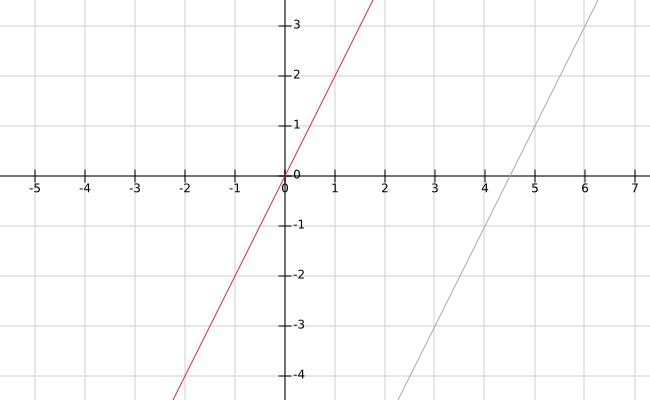
\includegraphics[scale=0.65]{graph_1_3_1.png} 

\textbf{4.} Ange ekvationen för en linje som är vinkelrät mot linjen $y=\dfrac{x}{3}-7$.

\textbf{Lösning}\\
I kurslitteraturen bevisas att två icke-vertikala linjer med riktningskoefficienterna $k_{1}$ och $k_{2}$ är vinkelräta om och endast om $k_{2} = -\dfrac{1}{k_{1}}$.

Vi har en given linje med riktningskoefficienten $k_{1} = \dfrac{1}{3}$. Det betyder att att en linje som är vinkelrät mot den givna linjen måste ha  riktningskoefficienten $k_{2}=-3$.

Den sökta linjens m-värde kan väljas godtyckligt. Vi väljer $m = 3$.

Ekvationen för den sökta linjen blir $y = -3x + 3$.

Som en extra kontroll väljer vi även att plotta ut dom två linjerna. I bilden nedan ser vi dom två linjerna. Linjerna ser hyfsat vinkelräta ut så vi har antagligen räknat rätt.

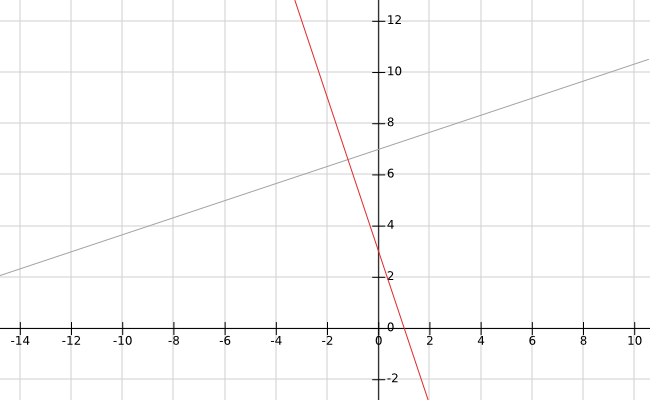
\includegraphics[scale=0.65]{graph_1_4_1.png}

\textbf{5.} Bestäm ekvationen för den linje som går genom punkterna $(2,\dfrac{7}{3})$ och $(-2,\dfrac{43}{3})$

\textbf{Lösning}\\
Vi börjar med att beräkna linjens riktningskoefficient.

$k=\dfrac{y_{2}-y_{1}}{x_{2}-x_{1}}=\dfrac{\dfrac{43}{3}-\dfrac{7}{3}}{-2-2}=\dfrac{\dfrac{36}{3}}{-4}=-\dfrac{12}{4}=-3$

Vi vet nu att linjen är på formen $y=-3x+m$. Återstår att bestämma värdet på $m$. Detta görs genom att sätta in en av dom givna punkterna i linjens ekvation.

$\dfrac{7}{3}=-3(2)+m$

$\dfrac{7}{3}=-6+m$

$m=\dfrac{7}{3}+6$

$m=\dfrac{7}{3}+\dfrac{18}{3}$

$m=\dfrac{25}{3}$

Den sökta linjens ekvation är alltså $y=-3x+\dfrac{25}{3}$

Vi väljer att kontrollera rimligheten på svaret genom att plotta linjen, se figuren nedan. Det ser ut som om dom två kända punkterna ligger på linjen så resultatet verkar rimligt.

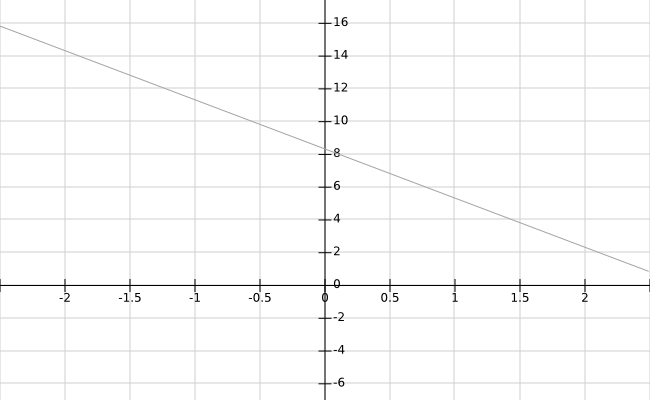
\includegraphics[scale=0.65]{graph_1_5_1.png}

\textbf{6.} Bestäm ekvationerna för de tre linjerna nedan.

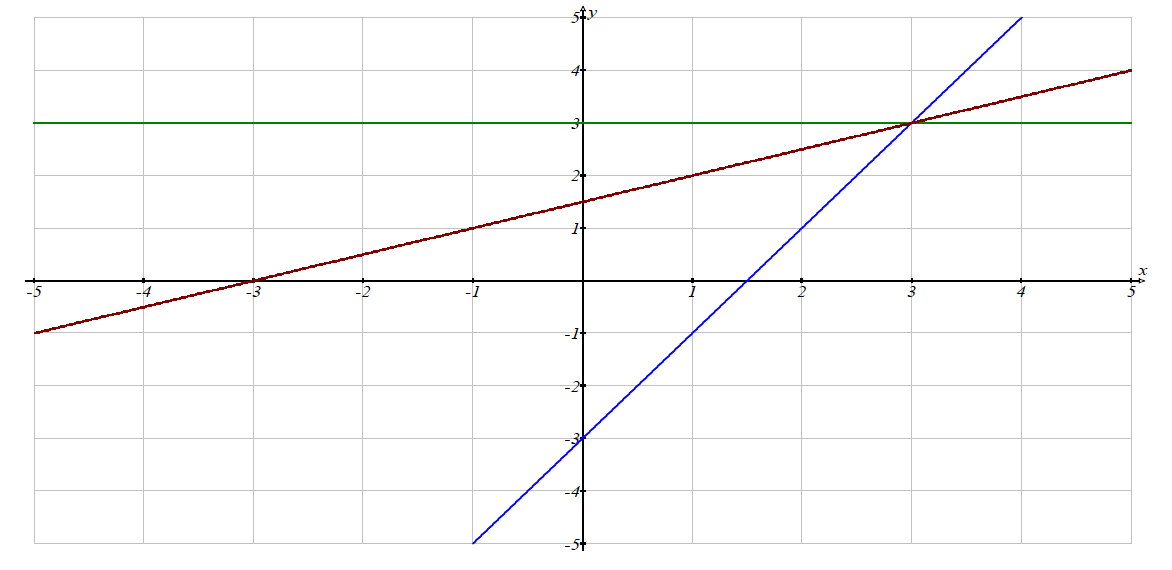
\includegraphics[scale=0.36]{graph_1_6_1.png}

\textbf{Lösning}

Man inser direkt att den gröna horisontella linjen beskrivs av ekvationen $y = 3$.

Vi väljer sedan att titta på den röda linjen. Man ser att två punkter på denna linjen är $(-3, 0)$ och $(3, 3)$. Med hjälp av dessa punkter kan vi räkna ut riktningskoefficienten $k$.

$k=\dfrac{3-0}{3-(-3)}=\dfrac{3}{6}=\dfrac{1}{2}$

Sätt nu in koordinaterna $(3, 3)$ och $k = \dfrac{1}{2}$ i räta linjens ekvation för att ta reda på värdet av $m$.

$y = kx + m$

$3 = \dfrac{1}{2}3 + m$

$m = 3 - \dfrac{3}{2}$

$m = \dfrac{3}{2}$

Vi vet nu att den röda linjen beskrivs av ekvationen $y = \dfrac{1}{2}x + \dfrac{3}{2}$

Till sist är det dags att titta på den brantaste blå linjen. Man ser att två punkter på denna linjen är $(0, -3)$ och $(3, 3)$. Med hjälp av dessa punkter kan vi räkna ut riktningskoefficienten $k$.

$k=\dfrac{3-(-3)}{0-(-3)}=\dfrac{6}{3}=2$

Sätt nu in koordinaterna $(3, 3)$ och $k = 2$ i räta linjens ekvation för att ta reda på värdet av $m$.

$y = kx + m$

$3 = 2\cdot3 + m$

$m = 3 - 6$

$m = -3$

Vi vet nu att den röda linjen beskrivs av ekvationen $y = 2x - 3$.
\end{document}
